\section{Eksperymenty}
\subsection{Klasyfikacja kNN - dobór liczby sąsiadów}
Dobór liczby sąsiadów dla algorytmu kNN jest bardzo istotny. Zbyt mała liczba sąsiadów może powodować zbytnie dopasowanie do danych, zbyt duża - negatywnie wpłynie na wartości dokładności i precyzji.\\

W celu optymalnego doboru k posłużyły średnie wartości dokładności z wykorzystaniem kroswalidacji (o podziale zbioru na 10). Następnie rysuję wykres średniej dokładności w zależności od liczby sąsiadów:

\begin{figure}[H]
    \centering
    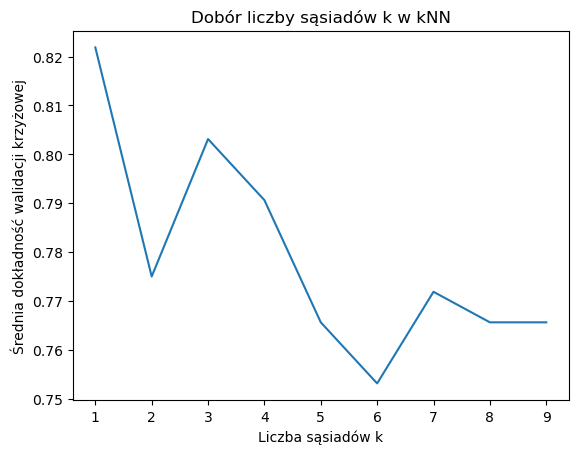
\includegraphics[scale=0.7]{knn_n}
    \caption{Wykres średniej dokładności walidacji krzyżowej}
    \label{fig:knn_n}
\end{figure}

Z obawy o zbytnie dopasowanie wybieram liczbę sąsiadów równą 3.

\subsection{Klasyfikacja kNN }
W przeprowadzonym eksperymencie dokonano podziału zbioru 80:20 (20 procent danych testowych). Następnie zdefiniowano klasyfikator z parametrem n\_neighbors równym 3. Kolejnym krokiem było wytrenowanie klasyfikatora i przeprowadzenie predykcji na zbiorze testowym:\\

\begin{lstlisting}[language=Python, caption=Definicja i użycie kNN]
from sklearn.neighbors import KNeighborsClassifier
from sklearn import metrics

knn = KNeighborsClassifier(n_neighbors=3)
knn.fit(X_train, y_train)
score = cross_val_score(knn, X_train, y_train, cv=10, scoring='accuracy')

y_pred = knn.predict(X_test)
\end{lstlisting}

\subsubsection{Wyniki}
Podstawowe metryki dla pierwszego eksperymentu wynosiły precyzja (\textit{Precision}): 0.90 a dokładność (\textit{Accuracy}): 0.7625. Średnia dokładność z użyciem walidacji krzyżowej (z podziałem zbioru testowego na 10) 0.803125. Co nie stanowi wiele informacji, korzystam więc z gotowych metryk dostępnych w bibliotece scikit-learn:\\

\begin{verbatim}
                             precision   recall f1-score  support

            Basilar-type aura     0.67     0.29     0.40        7
 Familial hemiplegic migraine     0.43     0.60     0.50        5
        Migraine without aura     0.71     0.62     0.67        8
                        Other     1.00     0.33     0.50        3
 Sporadic hemiplegic migraine     0.00     0.00     0.00        4
   Typical aura with migraine     0.81     0.96     0.88       49
Typical aura without migraine     1.00     0.75     0.86        4

                     accuracy                       0.76       80
                    macro avg     0.66     0.51     0.54       80
                 weighted avg     0.74     0.76     0.73       80
\end{verbatim}

W przypadku walidacji dla poszczególnych klas precyzja wahała się pomiędzy 43 a 100\%. Recall charakteryzował się dużym rozrzutem wartości - mniej liczne klasy miały recall niekiedy i 0-29\% a te bardziej liczne 75-96\%.\\

Średnia wartość recallu to 51\% a średnia ważona 76\% (ta właśnie uwzględniała nierówną liczebność klas). Podobna różnica miała miejsce w przypadku precyzji wyliczonej dla poszczególnych klas - średnia wartość 66\% - średnia ważona 74\%.\\

\subsection{Klasyfikacja Naiwnym Klasyfikatorem Bayesa}
W eksperymencie tym sprawdziłem wyniki klasyfikacji Naiwnym Klasyfikatorem Bayesa. Biblioteka scikit-learn umożliwia przeprowadzenie tzn \textit{Categorical Classication (Categorical Naive Bayes)} gdzie w przeciwieństwie do popularnej klasyfikacji binarnej, metoda jest w stanie zwrócić dwie informacje: etykietę klasy będącej wynikiem klasyfikacji oraz listę ze stopniami podobieństwa dla wszystkich klas.\\

\begin{lstlisting}[language=Python, caption=Definicja i użycie CategoricalNB]
from sklearn.naive_bayes import CategoricalNB

gnb = CategoricalNB()
    
y_pred = gnb.fit(X_train, y_train).predict(X_test)
\end{lstlisting}    

\subsubsection{Wyniki}
O ile wyniki dokładności (\textit{Accuracy}) wyglądały podobnie niz dla np. kNN - dokładnie 75\%. O tyle wyniki dla całości zbiory prezentowały się gorzej o 5-6 punktów procentowych niz dla kNN - precyzja średnia 64\% (względem 66\%) oraz precyzja wazona 69\% (względem 74\%). Wyniki dla poszczególnych klas dla precyzji potrafiły się różnić o 20-30 punktów procentowych względem kNN nie dając wyraźniej korelacji względem liczebności klas. Wyniki dla recall po trafiły być niekiedy diametralnie różne - 88\%-12\% a niekiedy znikomo - 92\%-96\% względem kNN.\\

\begin{verbatim}
                              precision  recall  f1-score   support

            Basilar-type aura      1.00    0.88      0.93         8
 Familial hemiplegic migraine      0.75    0.60      0.67         5
        Migraine without aura      0.29    0.18      0.22        11
                        Other      1.00    1.00      1.00         4
 Sporadic hemiplegic migraine      0.00    0.00      0.00         5
   Typical aura with migraine      0.76    0.92      0.83        62
Typical aura without migraine      0.67    0.40      0.50         5

                     accuracy                        0.75       100
                    macro avg      0.64    0.57      0.59       100
                 weighted avg      0.69    0.75      0.71       100
\end{verbatim}

Niezwykle istotną możliwością wykorzystania Naiwnego Klasyfikatora Bayesa było wyświetlenie podobieństwa testowanej klasy względem wszystkich klas.\\

Niektóre z klas (niekoniecznie te bardziej licznie) przedstawiały bardzo jednoznaczną klasyfikację, np:\\

\begin{verbatim}
    Other
    0.0009411289994916489: 	 Basilar-type aura
    0.00024106562936048384:  Familial hemiplegic migraine
    1.3757510137960067e-06:  Migraine without aura
    0.9987800638900048:      Other
    5.212399025390643e-06: 	 Sporadic hemiplegic migraine
    3.406207926665455e-08: 	 Typical aura with migraine
    3.111926902521578e-05: 	 Typical aura without migraine
\end{verbatim}

dla innych (często dla konkretnych jak np. Typical aura without migraine czy Migraine without aura) mieliśmy rozkłady bardzo zróżnicowane:

\begin{verbatim}
    Typical aura without migraine
    0.08048228203931468:    Basilar-type aura
    0.2633221828713967:     Familial hemiplegic migraine
    0.0009416760319083586:  Migraine without aura
    0.005682255909626338:   Other
    0.22367861315019222:    Sporadic hemiplegic migraine
    0.15361555787258202:    Typical aura with migraine
    0.2722774321249797:     Typical aura without migraine
\end{verbatim}
albo nawet niemal bilateralne:

\begin{verbatim}
    Migraine without aura
    0.000315062484758524:    Basilar-type aura
    0.0008466488192796888:   Familial hemiplegic migraine
    0.516090617842986:       Migraine without aura
    0.001079067159295874:    Other
    0.0038615304383266213:   Sporadic hemiplegic migraine
    0.4772101808065339:      Typical aura with migraine
    0.0005968924488194133:   Typical aura without migraine
\end{verbatim}

\subsection{Selekcja i ekstrakcja cech}
W czasie wykonanych eksperymentów wykorzystano dwa sposoby selekcji cech: SKB i RFE, oraz mechanizm wyodrębnienia cech PCA.\\

Definicja algorytmu selekcji cech SKB (czyli Select k Best), wybór k dziesięciu najlepszych i wyświetlenie nowych nazw cech:
\begin{lstlisting}[language=Python, caption=Definicja selektora SKB]
from sklearn.feature_selection import SelectKBest, chi2

skb = SelectKBest(chi2, k = 10)
X2 = skb.fit_transform(X, y)
\end{lstlisting}

Definicja selektora cech RFE (dla klasyfikatora SVC i redukcji do 10 cech):

\begin{lstlisting}[language=Python, caption=Definicja selektora RFE]
from sklearn.feature_selection import RFE

svc = SVC(kernel = 'linear')

rfe = RFE(estimator = svc, n_features_to_select = 10, step = 1)
X3 = rfe.fit_transform(X, y.values.ravel())
\end{lstlisting}

Definicja ekstraktora cech PCA (ekstrakcja do 4 cech).

\begin{lstlisting}[language=Python, caption=Definicja ekstraktora cech PCA]
from sklearn.decomposition import PCA

pca = PCA(n_components = 4)
X4 = pca.fit_transform(X)
\end{lstlisting}

\subsubsection{Wyniki}
Wyniki prezentowały się następująco:

\begin{verbatim}
Średnia dokładność klasyfikacji z wykorzystaniem klasyfikatora ...

    kNN wyniosła:                0.8024999999999999
    kNN i metody SKB wyniosła:   0.7825
    kNN i metody RFE wyniosła:   0.865
    kNN i metody PCA:            0.7

    SVC wyniosła:                0.8825
    SVC i metody SKB wyniosła:   0.8
    SVC i metody RFE wyniosła:   0.8825
    SVC i metody PCA:            0.735
\end{verbatim}

Co interesujące to właśnie dyskusyjny eksperyment klasyfikacji KNN z selekcją RFE poprawił wynik dla kNN o 8 punktów procentowych a np. SKB pogorszył go o dwa. W przypadku klasyfikatora SVC w/w metody albo nie zmieniły wyniku (RFE) albo pogorszyły wynik od 8-10 punktów procentowych.\\

Użyty zbiór nie był zbiorem licznym ani tez obliczenia na nim wykonywane nie wymagały dużych mocy obliczeniowych. Nie istniało zatem żadne uzasadnienie stosowania którejkolwiek z w/w metod ponieważ przy praktycznie zerowej optymalizacji otrzymywaliśmy gorsze wyniki.\\

\subsection{Perceptron wielowarstwowy}
Kolejnym z przeprowadzonych eksperymentów było użycie perceptronu wielowarstwowego. Podział zbioru to 75\% na dane treningowe i 25\% na dane testowe. Ponownie wykorzystaliśmy bibliotekę scikit-learn:

\begin{lstlisting}[language=Python, caption=Definicja perceptronu wielowarstwowego]
    from sklearn.neural_network import MLPClassifier
    mlp = MLPClassifier(hidden_layer_sizes=(6),
                         max_iter=50000, 
                         alpha=0.0001,
                         solver='adam',
                         activation= 'logistic', 
                         random_state=25,
                         tol=0.0000001)
\end{lstlisting}

Wyjaśnienie wykorzystanych parametrów:
\begin{enumerate}
    \item hidden\_layer\_sizes - ilość warstw ukrytych
    \item max\_iter - liczba epok
    \item alpha - współczynnik regularyzacji który zapobiega zjawisku przeuczenia
    \item solver - wybór algorytmu optymalizacji "adam".
    \item activation - wybór sigmoidalnej funkcji aktywacji
    \item random\_state - ziarno generatora liczb losowych
    \item tol - tolerancja dla kryterium stop. Algorytm zatrzymuje się, jeśli zmiana wyniku (kosztu) jest mniejsza niż ta wartość.
\end{enumerate}

\subsubsection{Wyniki}
Wyniki działania perceptronu okazały się zaskakująco dobre. Przy relatywnie niskiej ilości warstw ukrytych (6), przeciętnej ilości epok (50000) i popularnym optymalizatorze ("adam") osiągnęliśmy dokładność (Accuracy) na poziomie 94\% i średnią ważoną precyzję 95\%. Recall wahał się od 60\% do 100\% (przy średniej ważonej wartości 94\%) a współczynnik F1 od 75\% do 100\% (przy średniej ważonej wartości 93\%).\\
\begin{verbatim}
                              precision  recall f1-score  support

            Basilar-type aura      1.00    0.20     0.33        5
 Familial hemiplegic migraine      0.57    0.80     0.67        5
        Migraine without aura      1.00    1.00     1.00       12
                        Other      1.00    1.00     1.00        3
 Sporadic hemiplegic migraine      0.75    1.00     0.86        3
   Typical aura with migraine      0.97    0.99     0.98       67
Typical aura without migraine      1.00    1.00     1.00        5

                     accuracy                       0.94      100
                    macro avg      0.90    0.86     0.83      100
                 weighted avg      0.95    0.94     0.93      100

NN Accuracy =  0.94
\end{verbatim}

Przy mniejszej ilości epok (5000) takiej samej ilości warstw ukrytych (6) i tym samym optymalizatorze ("adam") osiągnęliśmy dokładność (Accuracy) na poziomie 96\% i średnią ważoną precyzję 97\%. Recall wahał się od 60\% do 100\% a współczynnik F1 od 75\% do 100\% (przy średniej ważonej wartości 96\%) z tym że biblioteka wyświetliła ostrzeżenie że optymalizator nie zakończył działania więc wyniki mogę byś nieoptymalne.\\

\begin{verbatim}
                              precision  recall f1-score  support

            Basilar-type aura      1.00    0.60     0.75        5
 Familial hemiplegic migraine      0.67    0.80     0.73        5
        Migraine without aura      1.00    1.00     1.00       12
                        Other      1.00    1.00     1.00        3
 Sporadic hemiplegic migraine      0.75    1.00     0.86        3
   Typical aura with migraine      0.99    0.99     0.99       67
Typical aura without migraine      1.00    1.00     1.00        5

                     accuracy                       0.96      100
                    macro avg      0.91    0.91     0.90      100
                 weighted avg      0.97    0.96     0.96      100

NN Accuracy =  0.96
\end{verbatim}

\subsection{Sieć głęboka z funkcją aktywacji Softmax}
Perceptron wielowarstwowy choć dawał świetne wyniki to jednak dawał wynik przynależności do najbardziej prawdopodobnej klasy. W zagadnieniu klasyfikacji bólów głowy interesującym byłoby pokazać wynik w postać stopnia podobieństwa przynależności do każdej z możliwych klas. Z pomocą przychodzi nam funkcja aktywacji Softmax i możliwość zastosowania jej w głębokich sieciach neuronowych.\\

W przypadku funkcji aktywacji Softmax konieczne jest uzycie enkodera etykiet klas - czy zamianę etykiet na przyporządkowane im liczby. Następnie w/w liczby zamieniamy na tzw. format hot-one czyli format gdzie danej liczbie przyporządkowujemy ciąg binarny zer oraz jednej jedynki w miejscu w szeregu odpowiadającym danej liczbie. Po testowej klasyfikacji musimy nasze wyniki zdekodować z powrotem do formatu etykiet. Wszystkie te operacje umożliwia nam biblioteka scikit-learn.\\

Do definicji sieci głębokiej używam biblioteki TensorFlow i jej części Keras.
\begin{lstlisting}[language=Python, caption=Definicja sieci głębokiej z funkcją aktywacji Softmax]
model=tf.keras.models.Sequential()
model.add(tf.keras.layers.Dense(64, activation='relu'))
model.add(tf.keras.layers.Dense(32, activation='relu'))
model.add(tf.keras.layers.Dense(num_classes, 
                                activation='softmax'))
model.build(input_shape=23)
model.compile(optimizer='Adam',
              loss='categorical_crossentropy',
              metrics=['accuracy'])
\end{lstlisting}

W powyższej definicji mamy:
\begin{enumerate}
    \item definicje modelu sekwencyjnego
    \item definicje warstwy gęstej (Dense, wszystkie neurony połączone) z 64 neuronami i funkcją aktywacji ReLU.
    \item definicje warstwy gęstej (Dense, wszystkie neurony połączone) z 32 neuronami i funkcją aktywacji ReLU. 
    \item definicje warstwy gęstej (Dense) z funkcją aktywacji Softmax.
    \item określenie ilości wejść - 23 bo tyle mamy cech.
    \item kompilację modelu z optymalizatorem "adam", określeniem funkcji straty "categorical\_crossentropy" i definicje metryk.
\end{enumerate}


Następnie rozpoczynam trenowanie modelu dla 50 epok, wydzielenie 20\% zbioru testowego na zbiór walidacyjny i zapis modelu:
\begin{lstlisting}[language=Python, caption=Definicja sieci głębokiej z funkcją aktywacji Softmax]
history = model.fit(X_train,
                    y_train_one_hot,
                    epochs=50,
                    verbose=1,
                    validation_split=0.2)
tf.keras.models.save_model(model,'../models/softmax.keras')
\end{lstlisting}


Wyświetlenie wykresu wartości funkcji straty i porównanie jej z wartością straty na zbioru walidacyjnego daje mi orientacyjną możliwość oceny słuszności doboru ilości epok.\\


\begin{figure}[h]
    \centering
    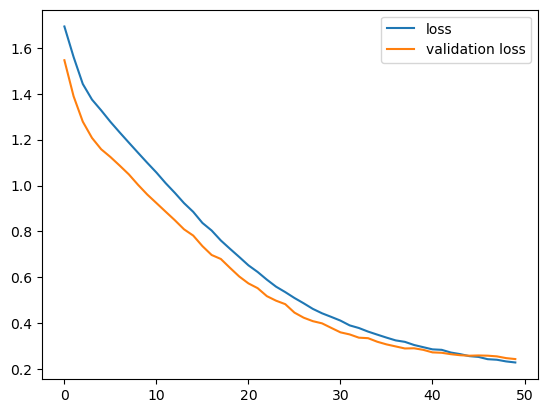
\includegraphics[scale=0.8]{valloss}
    \caption{Wykresy funkcji strat}
    \label{fig:valloss}
\end{figure}

\subsubsection{Wyniki}
Dla zbioru testowego osiągnęliśmy 95\% dokładność.\\

\begin{verbatim}
4/4 ==================== 0s 801us/step - accuracy: 0.9446 - loss: 0.2267
    Loss: 0.21024955809116364, Accuracy: 0.949999988079071
\end{verbatim}

Najciekawszym aspektem wykorzystania funkcji Softmax jest możliwość wyświetlenia podobieństwa do wszystkich możliwych klas. Oto kilka przykładów dla konkretnych przypadków, co zrobiłem na dwa sposoby. Pierwszy z nich wyświetlał wszystkie klasy i podobieństwa konkretnego przypadków do każdej z nich:\\

\begin{verbatim}
    Class: Basilar-type aura,             Probability: 0.25
    Class: Familial hemiplegic migraine,  Probability: 0.63
    Class: Migraine without aura,         Probability: 0.00
    Class: Other,                         Probability: 0.09
    Class: Sporadic hemiplegic migraine,  Probability: 0.03
    Class: Typical aura with migraine,    Probability: 0.00
    Class: Typical aura without migraine, Probability: 0.00
\end{verbatim}

a drugi z nich wyświetlał tabelę: enkodowana etykieta klasy, pełna etykieta klasy i prawdopodobieństwo do danej klasy analizowanego przypadku. Wartości uszeregowane malejąco wg podobieństwa:

\begin{verbatim}
                                Type  Probabilities
    1   Familial hemiplegic migraine           0.63
    0              Basilar-type aura           0.25
    3                          Other           0.09
    4   Sporadic hemiplegic migraine           0.03
    5     Typical aura with migraine           0.00
    6  Typical aura without migraine           0.00
    2          Migraine without aura           0.00
\end{verbatim}

\subsection{Prezentacja możliwości technik LIME dla NKB}
Techniki LIME zastosowano dla klasyfikacji Naiwnym Klasyfikatorem Bayesa. Ze względu na brak możliwości zastosowania normalizacji wyniki pracy z LIME prezentuje w osobnym podrozdziale jak i obliczenia przeprowadzono w osobnym arkuszu Jupytera.\\

\textbf{Przykład pierwszy: o niejednoznacznym rozkładzie podobieństw.}\\
\noindent W przykładzie widzimy niejednoznaczną klasyfikację. Najbardziej prawdopodobny wynik to "Typical aura with migraine" (59\%), drugi "Migraine without aura" (36\%). Listę klas z prawdopodobieństwami widzimy po lewej stronie wykresu rys. \ref{fig:lime_ex_1a}. Po środku niezbyt widoczny wykres wpływu cech na wynik. O tym szczegółowo poniżej. Po lewej stronie tabela z cechami i ich wartościami - uszeregowana wg istotności wpływu na wynik klasyfikacji. Wartości nie są znormalizowane co pokazuje np. wartość cechy Wiek ("Age").\\

\begin{figure}[H]
    \centering
    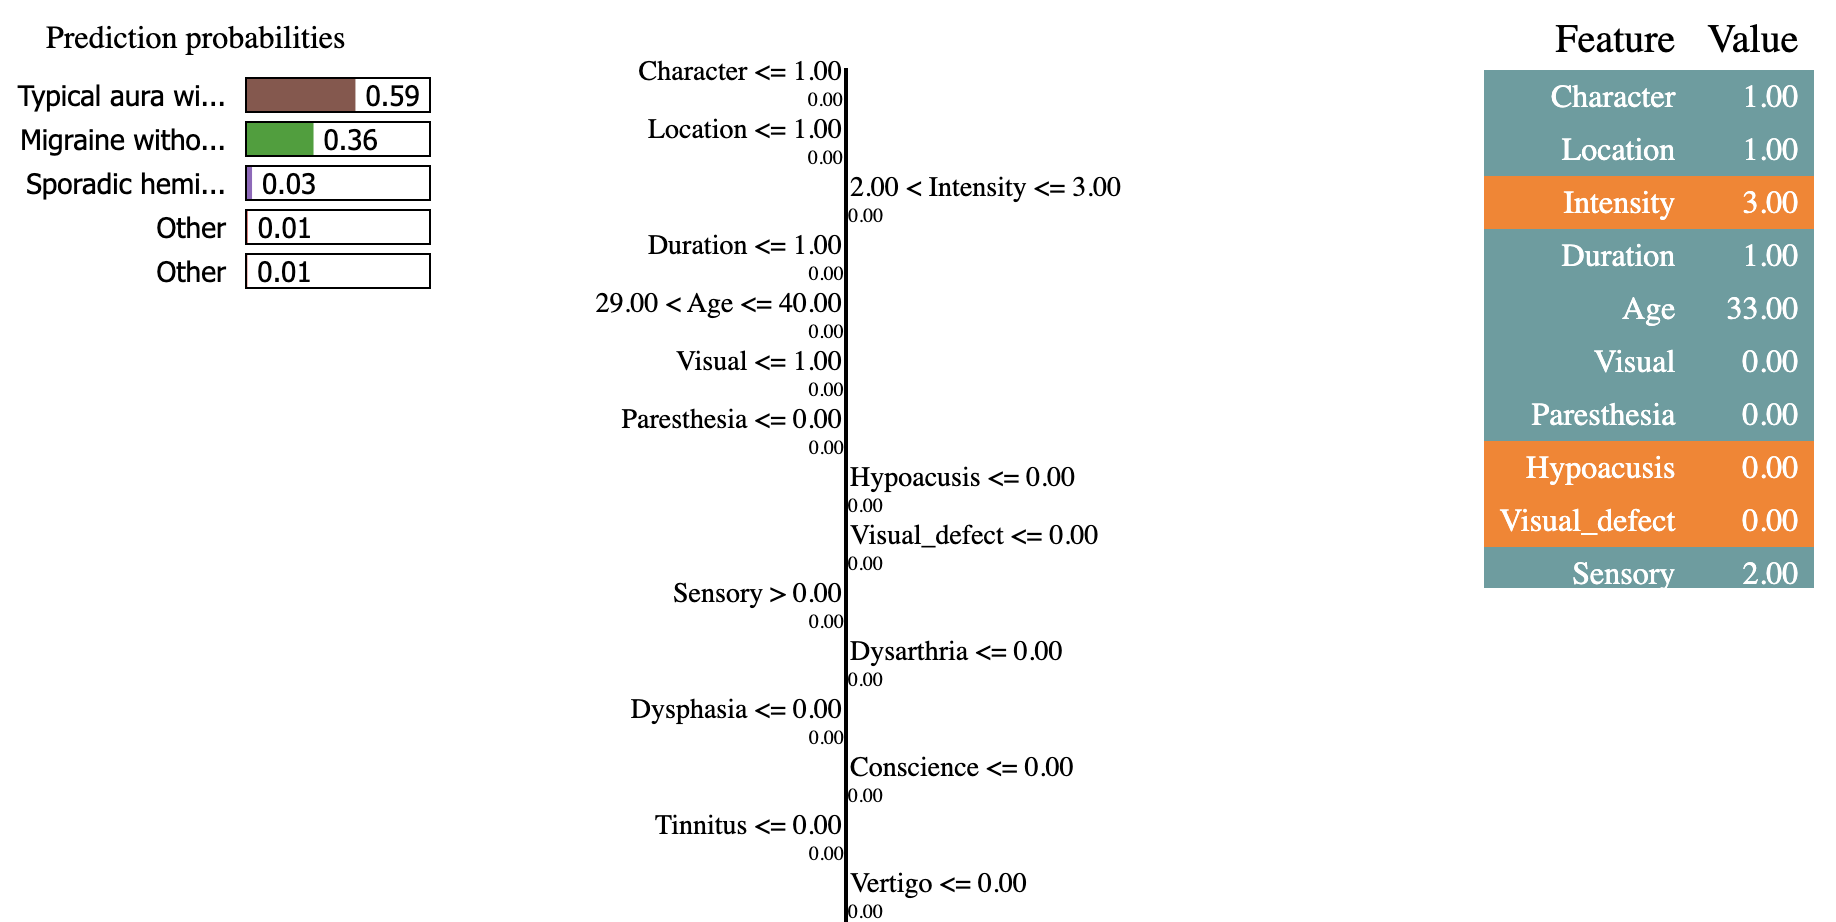
\includegraphics[scale=0.4]{lime_ex_1a}
    \caption{Zbiorcza prezentacja wyników LIME}
    \label{fig:lime_ex_1a}
\end{figure}

Poniżej bardziej czytelna wersja tabeli wpływu cech. Na osi poziomej widzimy orientacyjną wartość na cecha ta wpływała na wynik - zarówno jeśli cecha świadczyła za przynależnością do klasy (wartości dodatnie oznaczone na zielono) jak i wpływ cech przeciw klasyfikacji (ujemne wartości oznaczone na czerwono).\\

\begin{figure}[H]
    \centering
    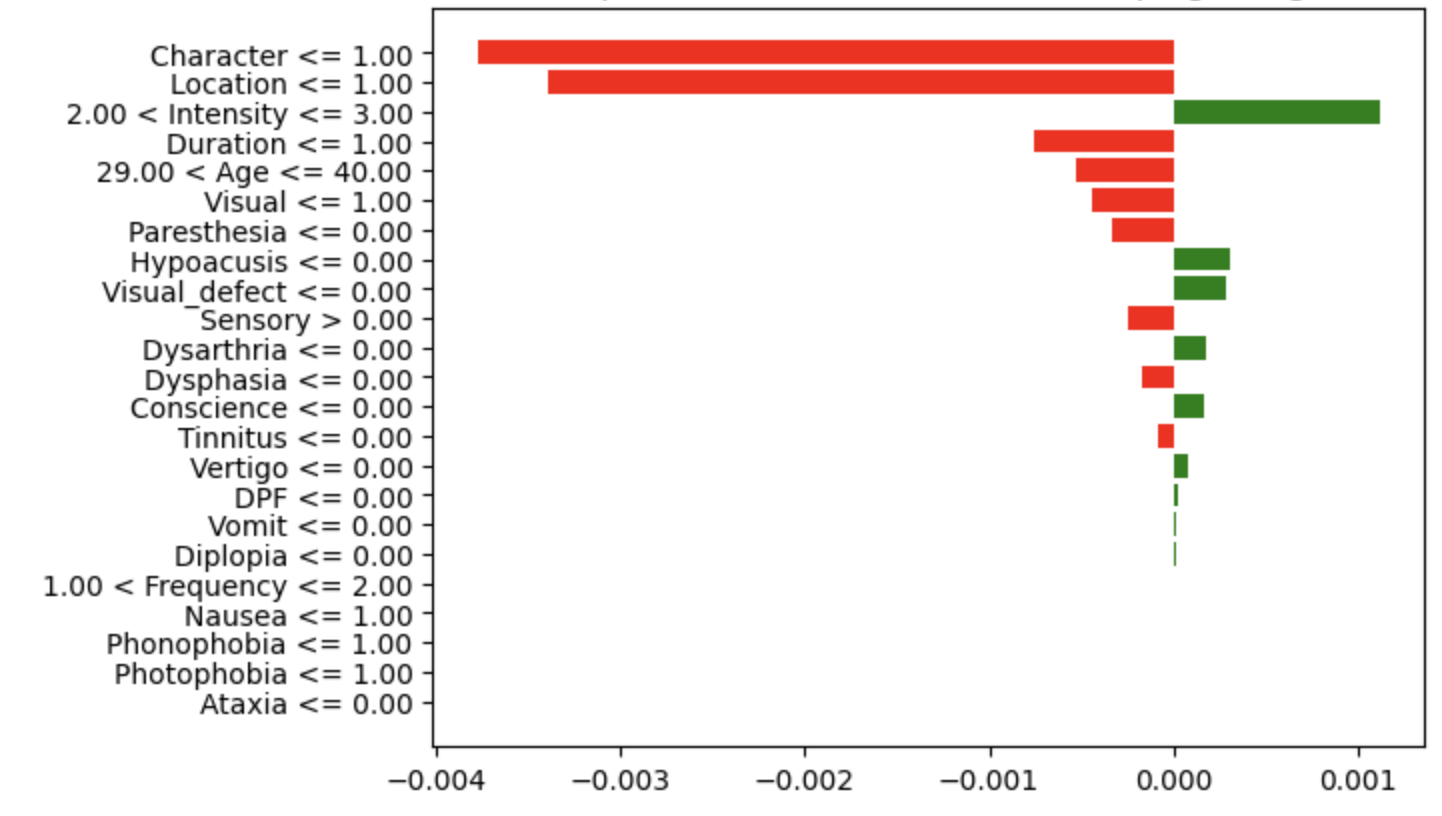
\includegraphics[scale=0.5]{lime_ex_1b}
    \caption{Szczegółowy rozkład wpływu cech na wynik}
    \label{fig:lime_ex_1b}
\end{figure}

W powyższym przykładzie widzimy że dwie najbardziej wpływowe cechy (charakter i lokalizacja) mogą świadczyć o przynależności wyniku do innej klasy a za klasyfikacją przemawia cecha nr 3 czyli intensywność bólu.\\

Pełne wyniki klasyfikacji algorytmem NKB prezentowały się zgodnie z wykresem z biblioteki LIME:

\begin{verbatim}
49 : Typical aura with migraine
0.0012638281303840333: 	Basilar-type aura
0.0059846389830973635: 	Familial hemiplegic migraine
0.363060881204291: 	    Migraine without aura
0.008800972062708684:   Other
0.032507610772455765:   Sporadic hemiplegic migraine
0.5883775288337598:     Typical aura with migraine
4.540013303382296e-06:  Typical aura without migraine
\end{verbatim}

\textbf{Przykład drugi: o jednoznacznym rozkładzie podobieństw.}\\
W drugim przykładzie przeanalizowano przykład o mocno jednoznacznym rozkładzie podobieństw (99\%).\\

\begin{figure}[H]
    \centering
    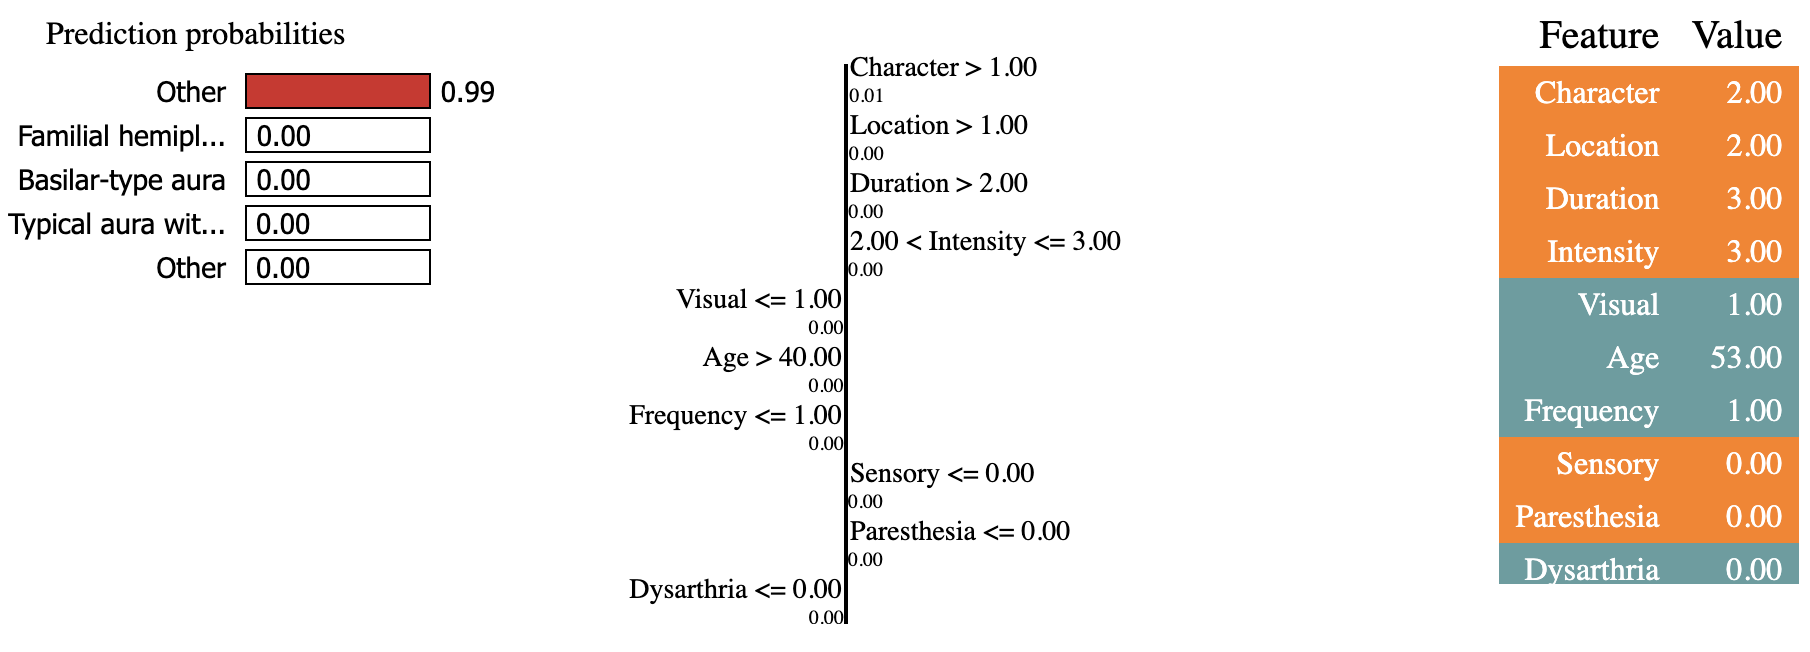
\includegraphics[scale=0.4]{lime_ex_2a}
    \caption{Zbiorcza prezentacja wyników LIME - 2}
    \label{fig:lime_ex_2a}
\end{figure}

Tutaj pierwsze cztery najbardziej dominujące cechy potwierdzają przynależność do klasy. Trzy kolejne poddają wynik pod wątpliwość.\\

\begin{figure}[H]
    \centering
    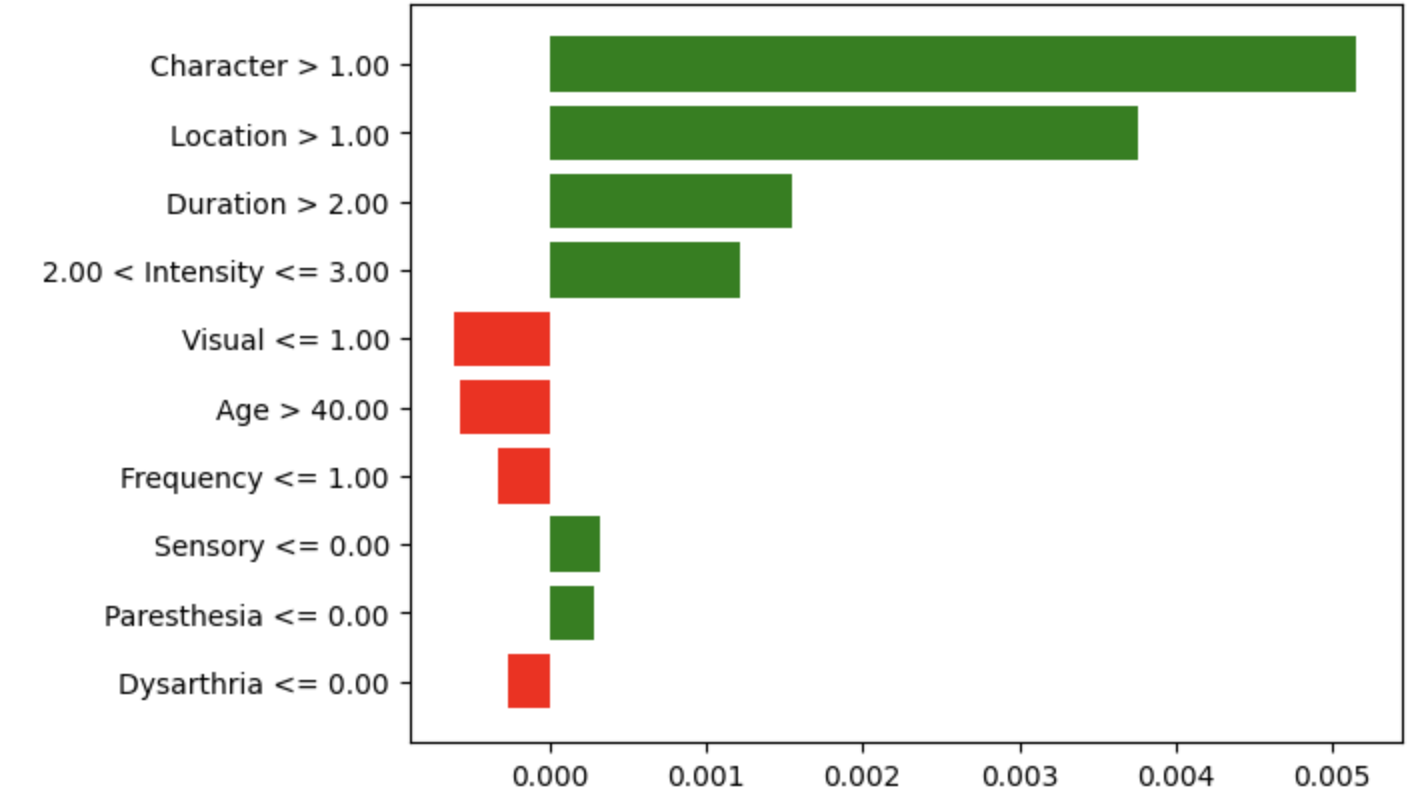
\includegraphics[scale=0.5]{lime_ex_2b}
    \caption{Szczegółowy rozkład wpływu cech na wynik - 2}
    \label{fig:lime_ex_2b}
\end{figure}

Prawdopodobieństwo potwierdzone przez wyniki NKB.\\

\textbf{Przykład trzeci: o jednoznacznym rozkładzie podobieństw.}\\
W drugim przykładzie przeanalizowano przykład o mocno jednoznacznym rozkładzie podobieństw (96\%).\\

\begin{figure}[H]
    \centering
    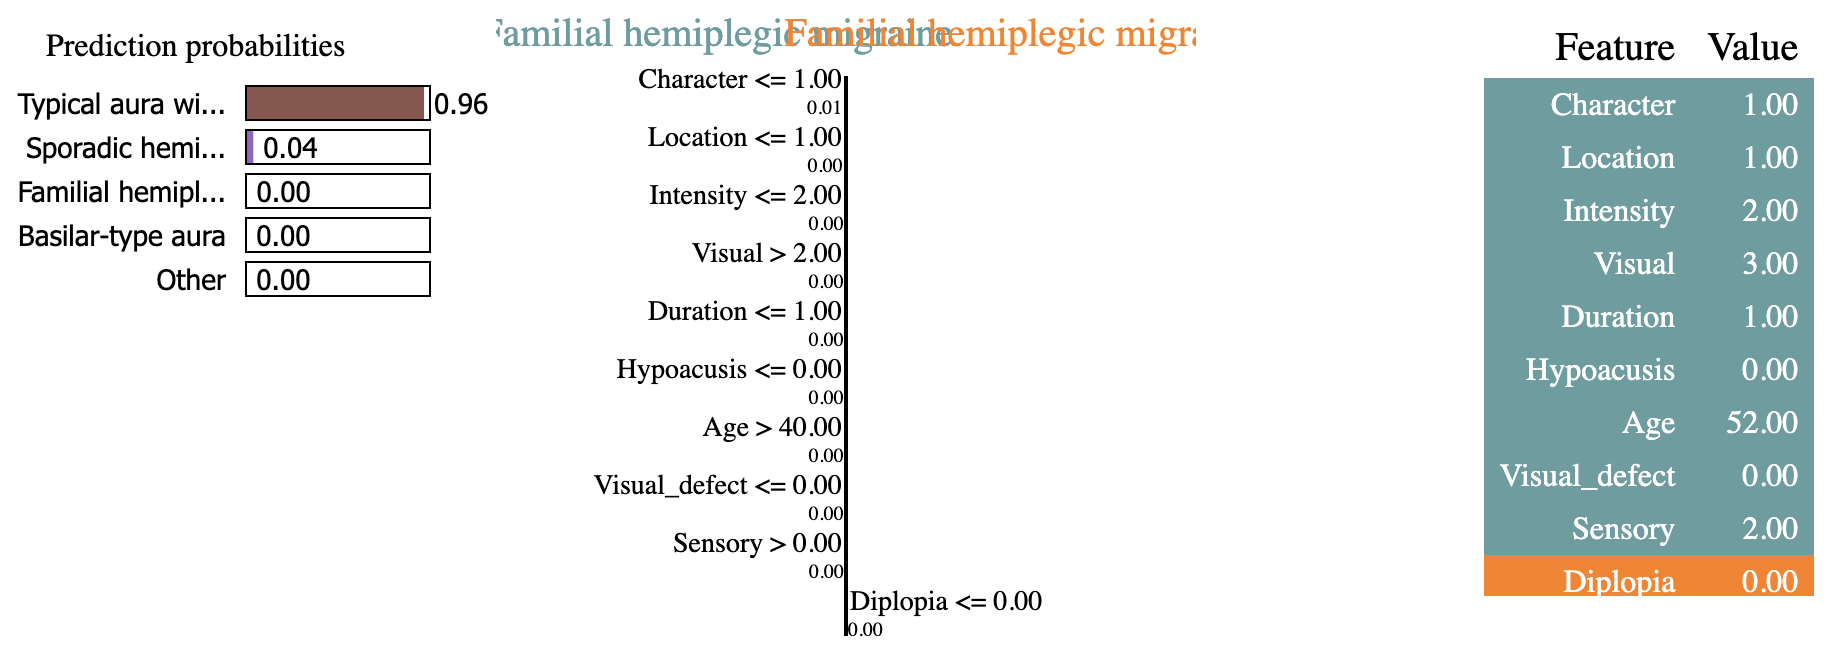
\includegraphics[scale=0.4]{lime_ex_3a}
    \caption{Zbiorcza prezentacja wyników LIME - 3}
    \label{fig:lime_ex_3a}
\end{figure}

Wynik jest o tyle interesujący że pomimo mocno jednoznacznej klasyfikacji aż dziewięć najbardziej dominujących klas sugeruje że instancja może należeć do innej klasy. W realnym przypadku taki wynik powinien być szczegółowo przeanalizowany przez osobę z ekspercką wiedzą domenową.\\

\begin{figure}[H]
    \centering
    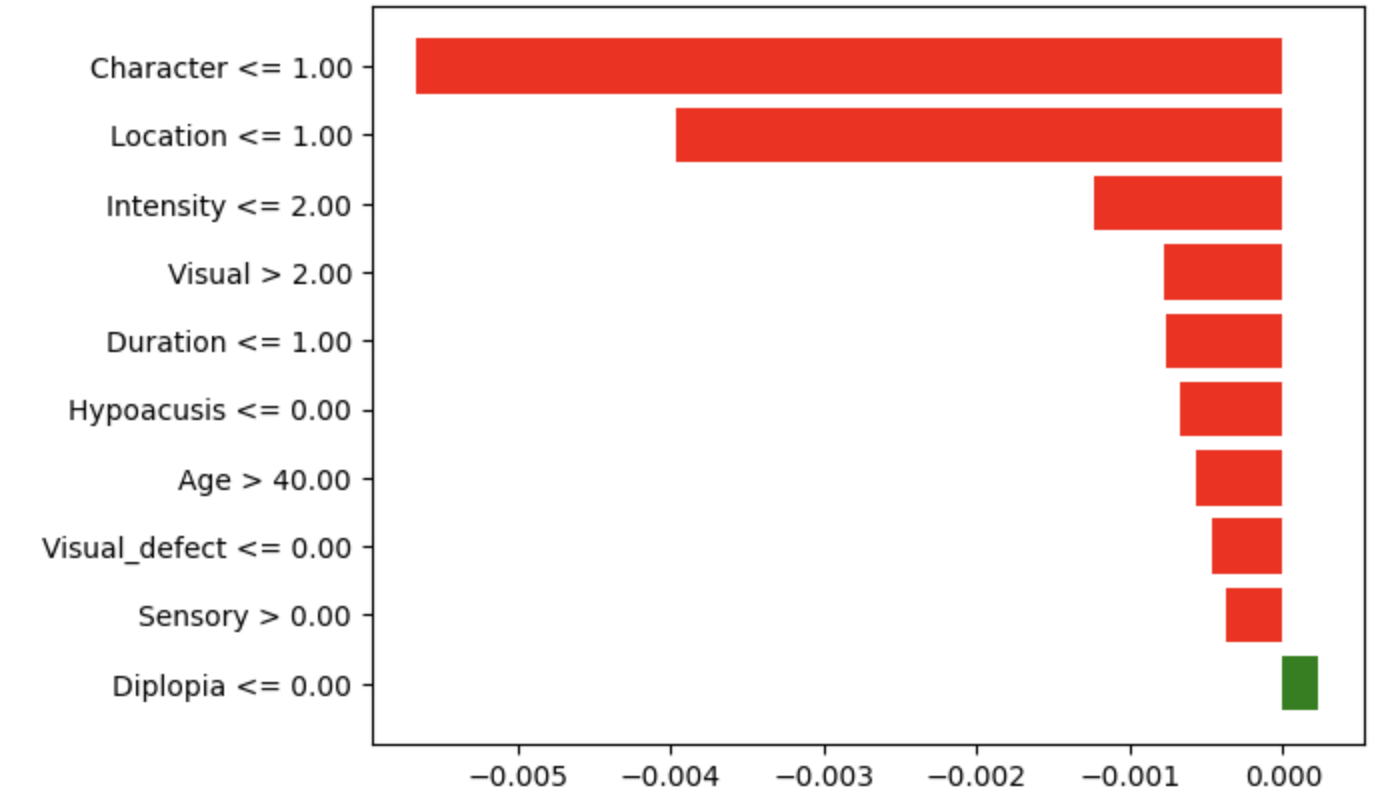
\includegraphics[scale=0.5]{lime_ex_3b}
    \caption{Szczegółowy rozkład wpływu cech na wynik - 3}
    \label{fig:lime_ex_3b}
\end{figure}

Prawdopodobieństwo potwierdzone przez wyniki NKB.\\

\subsection{Prezentacja możliwości technik SHAP dla NKB}
Techniki SHAP zastosowano również dla klasyfikacji Naiwnym Klasyfikatorem Bayesa. Zachowano taki sam podział zbioru i analizowano dokładnie taki sam zbiór testowy (w tym też konkretne przypadki). Tym razem również nie zastosowano normalizacji choć dla SHAP można ją stosować - zachowano te same warunki aby porównać wyniki.\\

\begin{lstlisting}[language=Python, caption=Definicja explainera dla SHAP]
# Funkcja predykcyjna modelu
def predict_proba(X):
    return gnb.predict_proba(X)

# Tworzenie wyjasniacza KernelExplainer
explainer = shap.KernelExplainer(predict_proba, X_train)

# Wybor jednej instancji ze zbioru testowego
instance = X_test.iloc[0].values.reshape(1, -1)

# Obliczanie wartosci SHAP dla wybranej instancji
shap_values = explainer.shap_values(instance)

# Tworzenie wykresu typu waterfall dla wybranej instancji i pierwszej klasy
shap.waterfall_plot(shap.Explanation(values=shap_values[0][0], 
                                base_values=explainer.expected_value[0], 
                                data=instance[0], 
                                feature_names=df.columns))
\end{lstlisting}

\begin{figure}[H]
    \centering
    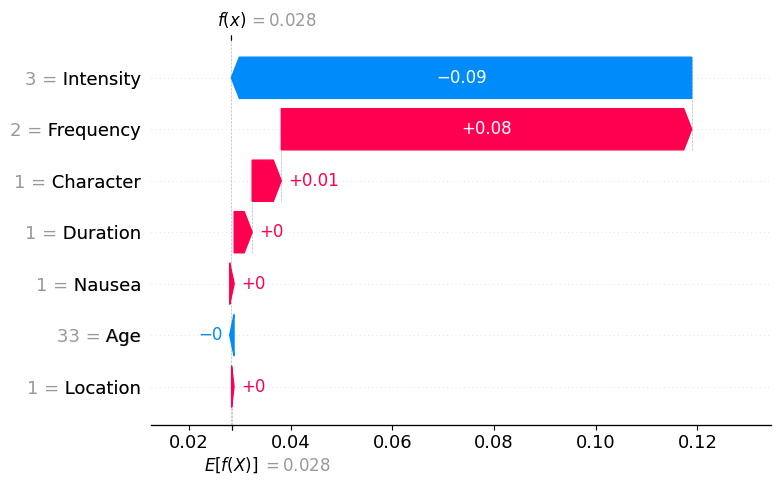
\includegraphics[scale=0.7]{shap_b_01}
    \caption{Wpływ cech wg SHAP dla NKB}
    \label{fig:shap_b_01}
\end{figure}
Dla porównanie przypomnienie wykresu dla LIME:

\begin{figure}[H]
    \centering
    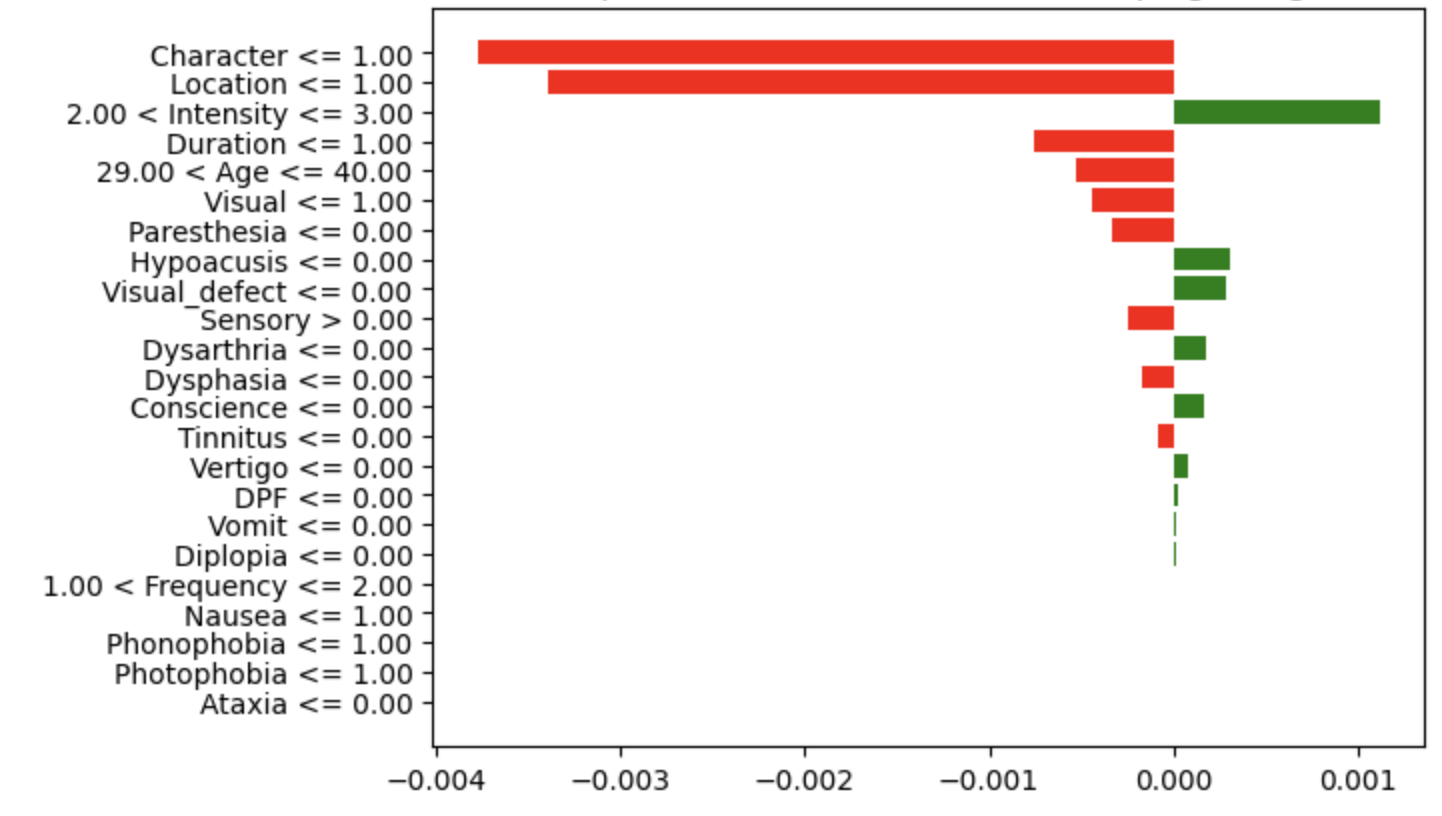
\includegraphics[width=0.9\textwidth]{lime_ex_1b}
\end{figure}

Widzimy częściową zgodność cech. Kolejność jak ich wartości wpływu są już praktycznie zupełnie różne.\\

Podobną sytuację obserwujemy dla pozostałych przypadków:
\begin{figure}[H]
    \centering
    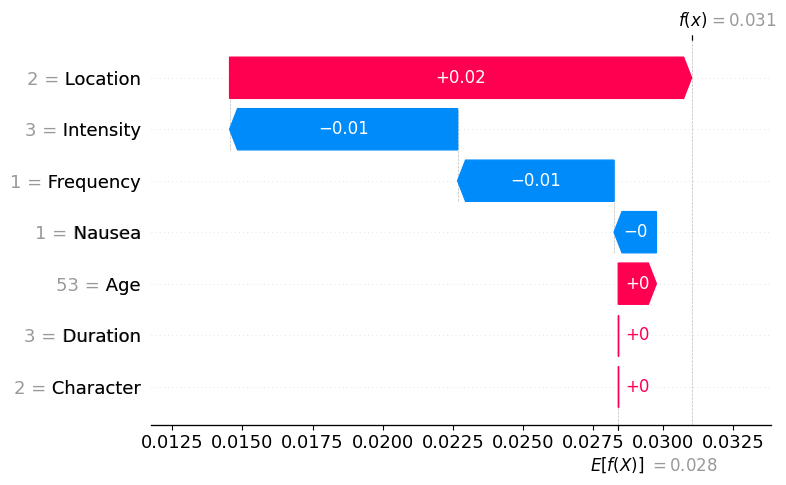
\includegraphics[scale=0.7]{shap_b_02}
    \caption{Wpływ cech wg SHAP dla NKB - 2}
    \label{fig:shap_b_02}
\end{figure}
Dla porównanie przypomnienie wykresu dla LIME:

\begin{figure}[H]
    \centering
    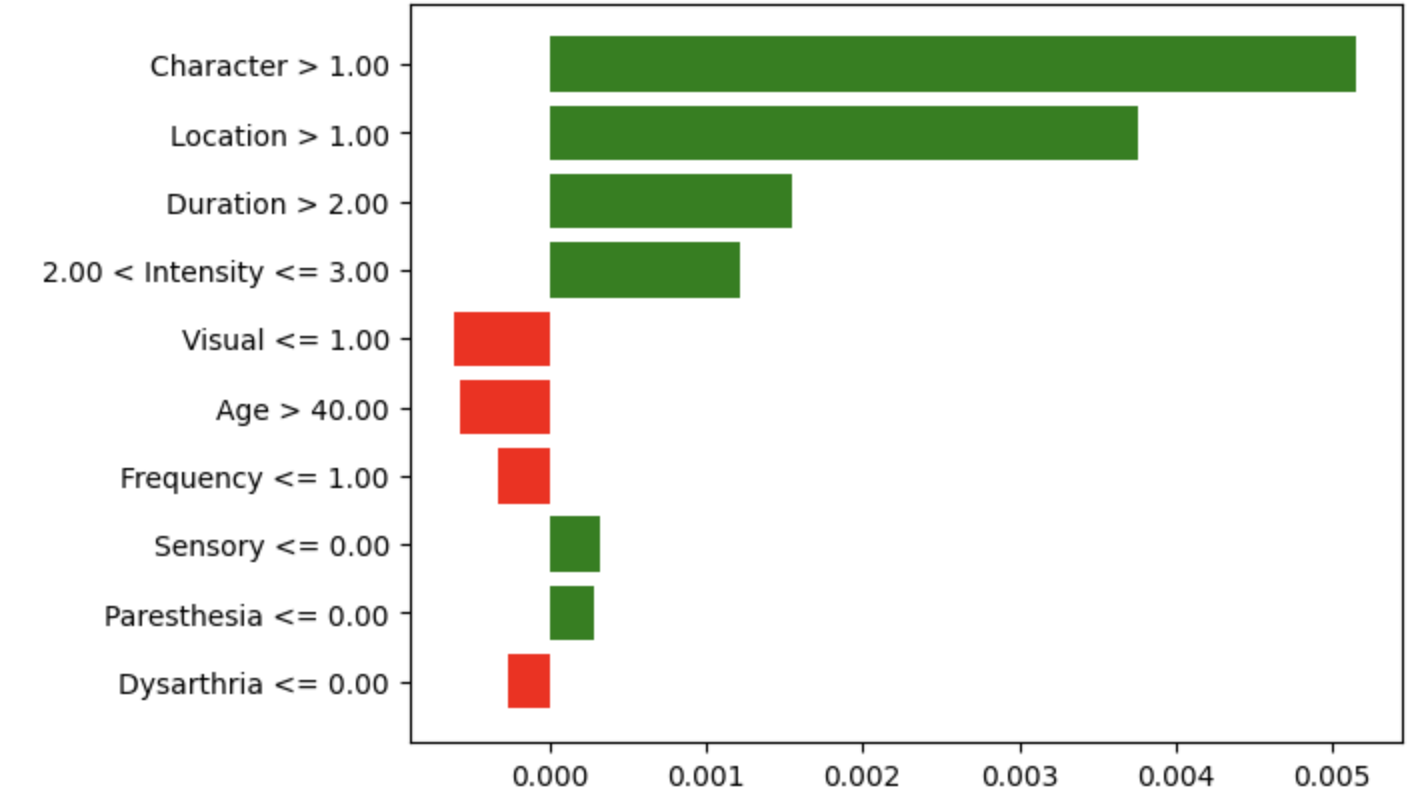
\includegraphics[width=0.9\textwidth]{lime_ex_2b}
\end{figure}

Kolejny przykład:
\begin{figure}[H]
    \centering
    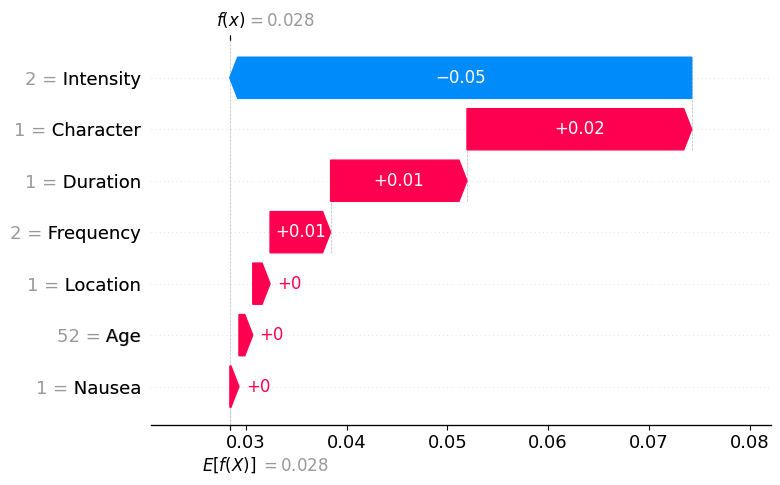
\includegraphics[scale=0.7]{shap_b_03}
    \caption{Wpływ cech wg SHAP dla NKB - 3}
    \label{fig:shap_b_03}
\end{figure}
Dla porównanie przypomnienie wykresu dla LIME:

\begin{figure}[H]
    \centering
    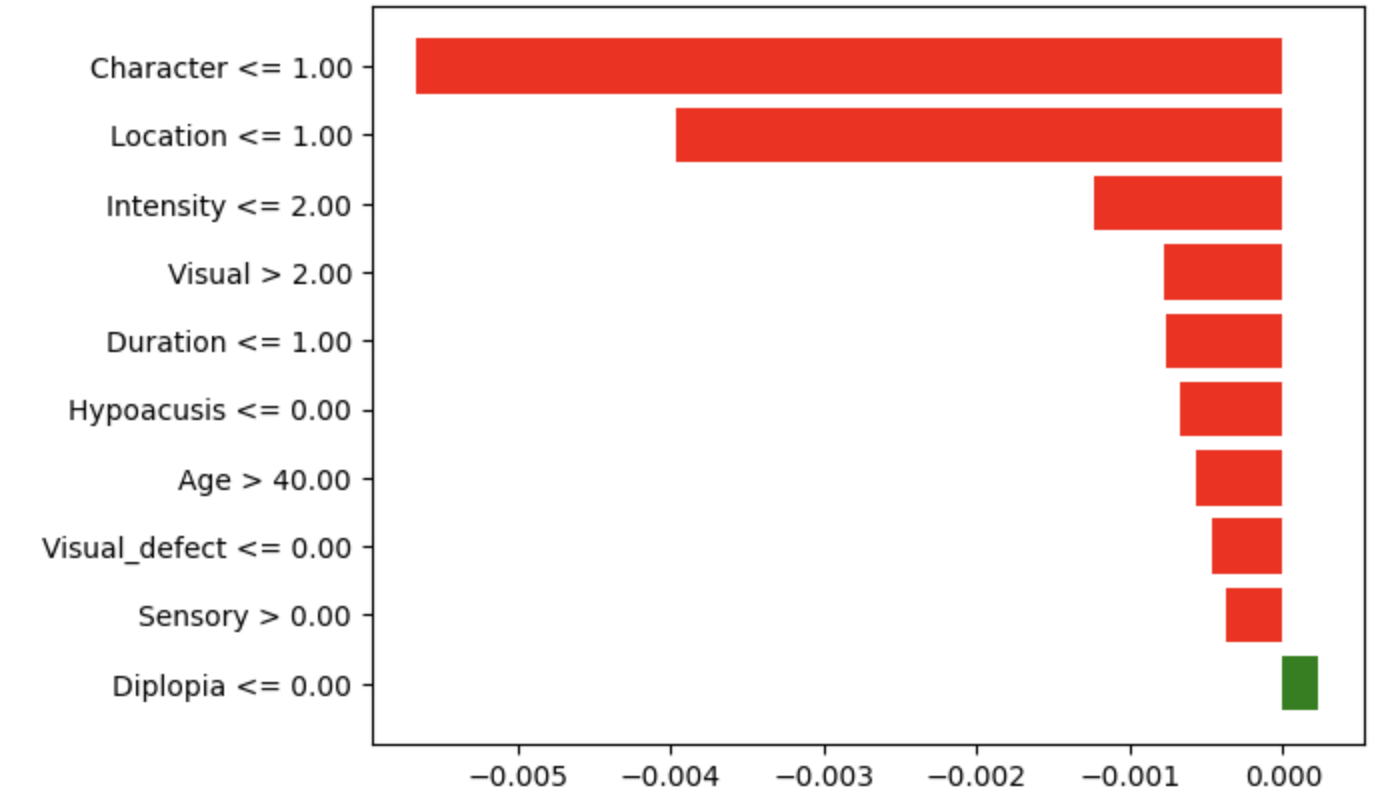
\includegraphics[width=0.9\textwidth]{lime_ex_3b}
\end{figure}


\subsection{Prezentacja możliwości technik SHAP dla sieci głębokiej}
Techniki SHAP zastosowano też dla głębokiej sieci neuronowej. Pomimo zastosowania takiego samego podziału zbioru i dokładnie takiego samego zbioru testowego (w tym już konkretnych przypadków) wyniki znacznie różniły się od wyników dla LIME.\\

Definicja "wyjaśniacza" jest tutaj nieco trudniejsza niż dla LIME i nieco mniej intuicyjna (choćby przez konieczność dwukrotnej definicji numeru interpretowanej instancji):

\begin{lstlisting}[language=Python, caption=Definicja explainera dla SHAP - 2]
# Tworzenie wyjasniacza KernelExplainer
explainer = shap.KernelExplainer(predict, X_train)
    
# Obliczanie wartosci SHAP dla przykladowych danych
shap_values = explainer.shap_values(X_test[0:1])  # X_test to dane testowe, wybieramy przyklad 0
    
# Tworzenie obiektu Explanation z etykietami cech
explanation = shap.Explanation(values=shap_values[0][0], 
                           base_values=explainer.expected_value[0], 
                           data=X_test[0],
                           feature_names=df.columns)
    
# Wyswietlanie wykresu wodospadowego
shap.waterfall_plot(explanation)
\end{lstlisting}

\begin{figure}[H]
    \centering
    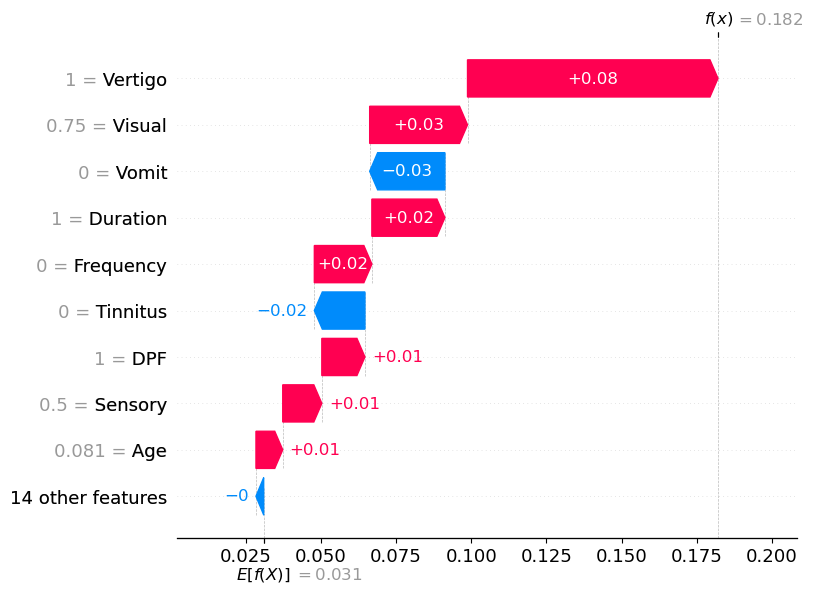
\includegraphics[scale=0.5]{shap_d_01}
    \caption{Wpływ cech wg SHAP dla sieci}
    \label{fig:shap_d_01}
\end{figure}

\begin{figure}[H]
    \centering
    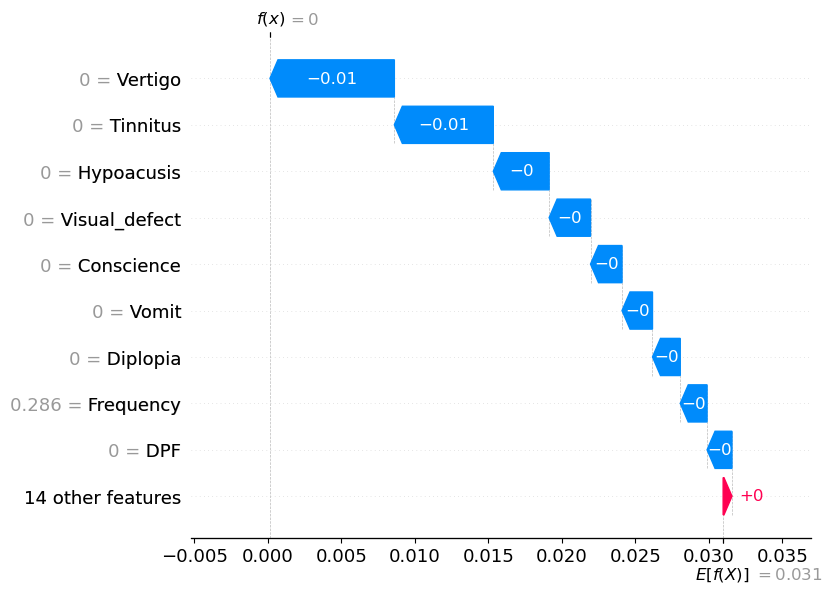
\includegraphics[scale=0.5]{shap_d_02}
    \caption{Wpływ cech wg SHAP dla sieci - 2}
    \label{fig:shap_d_02}
\end{figure}

\begin{figure}[H]
    \centering
    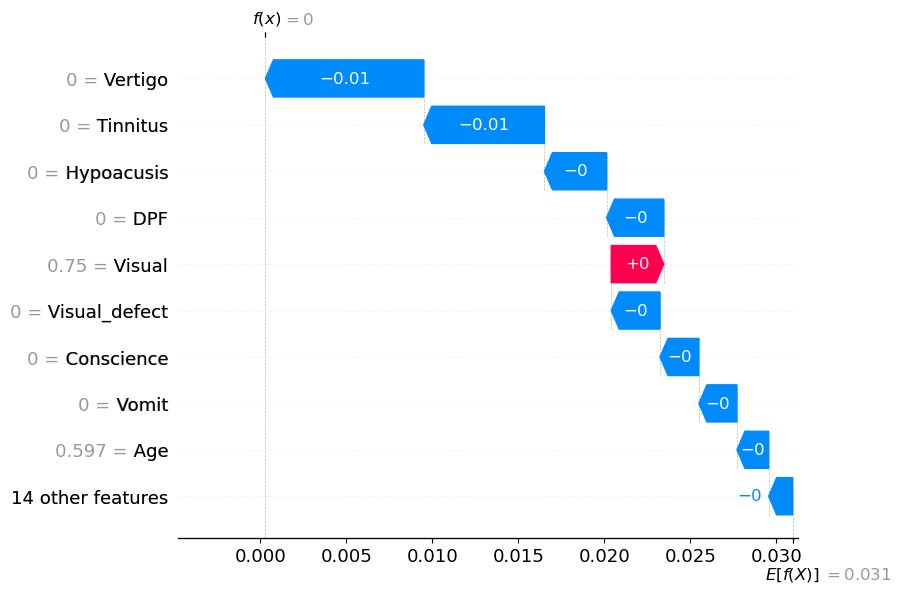
\includegraphics[scale=0.5]{shap_d_03}
    \caption{Wpływ cech wg SHAP dla sieci - 3}
    \label{fig:shap_d_03}
\end{figure}

Powyższe wykresy to tzw. wykresy wodospadowe.\\
\noindent\textbf{Oś Y - Cechy} - Lista cech (np. Vertigo, Hypoacusis, Conscience) znajduje się po lewej stronie wykresu. Każda cecha ma przypisaną wartość z danych wejściowych (np. 0 = Vertigo).\\
\noindent\textbf{Oś X - Wartości SHAP} - Oś X przedstawia wartości SHAP, które pokazują wpływ każdej cechy na końcową przewidywaną wartość modelu. Wartości SHAP są liczbami, które mogą być dodatnie lub ujemne.\\

\textbf{Kolory:}\\
\noindent\textbf{Niebieski:} Negatywny wpływ na przewidywanie (obniżają wartość przewidywaną przez model).\\
\noindent\textbf{Czerwony:} Pozytywny wpływ na przewidywanie (zwiększają wartość przewidywaną przez model).\\

Wartości SHAP pokazują, jak poszczególne cechy wpływają na wynik przewidywany przez model.
Cechy z największymi wartościami SHAP (pozytywnymi lub negatywnymi) mają największy wpływ na decyzję modelu.
Wartość bazowa reprezentuje średnią przewidywaną wartość na podstawie danych treningowych, a przewidywana wartość f(x) pokazuje, jak daleko od tej średniej znajduje się przewidywanie dla konkretnego przykładu.\\

W Przypadku LIME cechami dominującymi zwykle były Character, Location, Duation, Intensity czy Age. Dla SHAP dominuje Vertigo, Tinnitus, Visual czy Vomit. Ze względu na różne algorytmy decyzyjne (Naiwny Klasyfikator Bayesa i Głęboka Sieć Neuronowa) porównanie wyników obu technik dla tych samych instancji zdaję się nie mieć sensu, co jednocześnie nie przekreśla użycia obu technik w konsultacji z osobą z wiedzą domenową w zaskresie medycyny bólów głowy.